\documentclass{article}
 
% PAQUETES
\usepackage{float}
\usepackage{amsmath}
\usepackage{graphicx}
\usepackage{tabularx}

\usepackage[spanish]{babel}
\usepackage[a4paper,top=2cm,bottom=2cm,left=3cm,right=3cm,marginparwidth=1.75cm]{geometry}
\usepackage[colorlinks=true, allcolors=blue]{hyperref}

% MODIFICADORES

\providecommand{\keywords}[1]{\textbf{\textit{Palabras clave---}} #1}

\linespread{1.3}
\setlength{\parskip}{2.5mm}
\setlength{\parindent}{0mm}

% TÍTULO DEL DOCUMENTO

\title{Identificación Semiautomática de Glaciares en Imágenes Satelitales Usando Técnicas de Inteligencia Artificial, Una Revisión Sistemática}
\author{William Condori Quispe} 

% DOCUMENTO

\begin{document}
\maketitle

\begin{abstract}

    La presente revisión sistemática tiene como objetivo identificar las tendencias de aplicación de técnicas basadas en inteligencia artificial para la identificación semi automática de glaciares usando imágenes satelitales. Para ello se ha hecho un análisis del estado del arte utilizando la metodología PRISMA para estudios publicados en los últimos cinco años ($>2017$). Se propusieron 9 preguntas de investigación cuya finalidad fue la identificación de los tipos de glaciares que se buscaron identificar, la composición de los conjuntos de datos, algoritmos empleados, estrategias de ejecución, y métricas de evaluación. La búsqueda de estudios se realizó sobre diferentes bases de datos indexadas, dando como resultado un total de 431 artículos encontrados. Posteriormente, se hizo un análisis para eliminar los resultados duplicados, así como también, los resultados cuyo título o resumen no guarden una relación directa con el objetivo planteado inicialmente. El proceso de filtrado de resultados concluyó con la selección de un total de 31 artículos de investigación, luego de la aplicación de criterios de elegibilidad y de exclusión. Finalmente, se enumeraron los estudios seleccionados y se procedió a responder las preguntas de investigación. El análisis de las respuestas permitió identificar el estado actual de la aplicación de técnicas basadas en inteligencia artificial en la identificación semiautomática de glaciares usando imágenes satelitáles.
\end{abstract}

\keywords{
    Revisión Sistemática,
    Identificación,
    Glaciares,
    Imagen satelital,
    Inteligencia Artificial,
    Machine Learning,
    Deep Learning
}


\section{Introducción}

Los glaciares son muy importantes para los ecosistemas de la Tierra, porque son una fuente de agua y una fuente de energía. Por ello, se ha desarrollado una serie de técnicas de identificación semi automática de glaciares en imágenes satelitales.

\section{Antecedentes y trabajos relacionados}

% =========================================================================
% METODOLOGÍA DE LA INVESTIGACIÓN
% =========================================================================

\section{Research methodology}

Esta revisión sistemática fue elaborada siguiendo la metodología PRISMA (Preferred Reporting Items for Systematic Review and Meta-Analysis), la cual establece un estandar para el proceso de identificación, selección, evaluación  y análisis del estado del arte.

\subsection{Objetivo de investigación}

comparar las diferentes metodologías propuestas, así como identificar las tendencias de uso en la aplicación de técnicas basadas en inteligencia artificial (Machine Learning/Deep Learning) en la identificación semi automática de glaciares usando imágenes satelitales.

\begin{figure}[H]
    \centering
    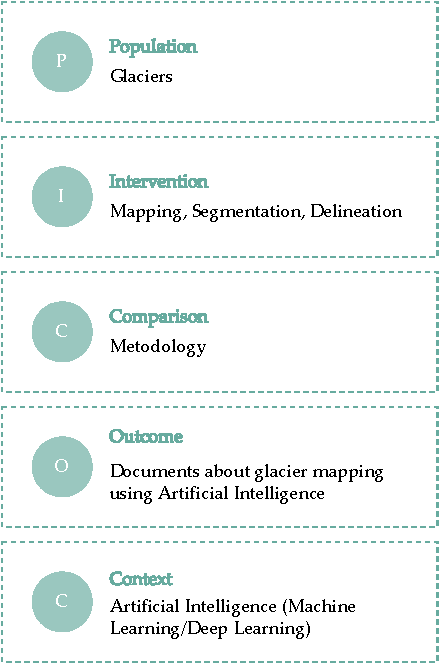
\includegraphics[width=0.4\textwidth]{images/picoc.pdf}
    \label{fig:picoc}
    \caption{Criterio PICOC empleado para delimitar el alcance y el objetivo de la revisión sistemática}
\end{figure}

\subsection{Research questions}

Las preguntas de investigación tuvieron como objetivo recopilar la información más destacada de cada estudio. Para esta revisión sistemática se han planteado seis preguntas de investigación, relacionadas con los siguientes aspectos:

\begin{itemize}
    \item Conjunto de datos.
    \item Tipos de glaciares y regiones de estudio.
    \item Algoritmos empleados y métricas de evaluación.
\end{itemize}

En la Tabla \ref{tab:research_questions} se han enumerado las preguntas planteadas y su correspondiente motivación.

\begin{table}[H]
    \centering
    \caption{Preguntas de investigación}
    \hspace{1cm}
    \label{tab:research_questions}
    \begin{tabularx}{\textwidth}{cXX}
        \hline
        \textbf{No.} & \textbf{Research Questions}                                                                    & \textbf{Motivations}                                                                                                                                                                                              \\ \hline
        RQ1          & ¿Qué imágenes satélites conformaron el conjunto de datos?                                      & Se buscó identificar el sensor de origen de las imágenes satelitales empleadas en la construcción del conjunto de datos utilizado en el trabajo de investigación.                                                 \\ \hline
        RQ2          & ¿Cuántas imágenes satelitales/muestras se utilizaron en la construcción del conjunto de datos? & Se buscó identificar el tamaño del conjunto de datos utilizado en el estudio para analizar el comportamiento del algoritmo empleado y posibles estrategias de incremento de datos en caso el tamaño sea reducido. \\ \hline
        RQ3          & ¿Qué tipo de glaciar se buscó identificar en el estudio?                                       & Esta pregunta permitió identificar la estrategia elegida por los autores para abordar la identificación de un tipo de glaciar específico considerando todas sus características inherentes.                       \\ \hline
        RQ4          & ¿Cuál es la región geográfica de estudio?                                                      &                                                                                                                                                                                                                   \\ \hline
        RQ5          & ¿Qué algoritmo de inteligencia artificial se empleó como base del modelo propuesto?            & Es la pregunta principal, ya que permitió identificar las tendencias de uso de los algoritmos de inteligencia artificial respecto al problema de visión por computador y los diferentes tipos de glaciares.       \\ \hline
        RQ6          & ¿Cuáles fueron las métricas utilizadas para la evaluación del modelo?                          & Se buscó identificar las métricas más utilizadas en la evaluación de modelos basados en inteligencia artificial para la identificación semiautomática de glaciares en imágenes satelitales.                       \\ \hline
    \end{tabularx}
\end{table}

\subsection{Source selection}

Luego de la definición de las preguntas de investigación, se seleccionaron las bases de datos más relevantes para la búsqueda de estudios en base a revisiones sistemáticas existentes relacionadas a la percepción remota y la inteligencia artificial [], ya que estas fueron las que más se ajustaron a las necesidades del estudio.

\begin{table}[H]
    \centering
    \caption{Bases de datos seleccionadas para la búsqueda de estudios}
    \hspace{1cm}
    \label{tab:selected_repositories}
    \begin{tabularx}{\textwidth}{XX}
        \hline
        arXiv             & \url{https://arxiv.org}           \\ \hline
        IEEE Xplore       & \url{https://ieeexplore.ieee.org} \\ \hline
        MDPI              & \url{https://mdpi.com}            \\ \hline
        Nature            & \url{https://nature.com}          \\ \hline
        Science Direct    & \url{https://sciencedirect.com}   \\ \hline
        Scopus            & \url{https://scopus.com}          \\ \hline
        Springer Link     & \url{https://link.springer.com}   \\ \hline
        Taylor \& Francis & \url{https://tandfonline.com}     \\ \hline
        Web of Science    & \url{https://isiknowledge.com}    \\ \hline
    \end{tabularx}
\end{table}

\subsection{Search Strategy}

Se ha empleado una estrategia de búsqueda primaria para la recopilación de estudios relacionados al objetivo de la revisión sistemática.

\textit{Primary search:} (“glacier” OR “glacial”) AND (“mapping” OR “delineation” OR “detection” OR “segmentation”) AND (“artificial intelligence” OR “machine learning” OR “deep learning”).

\begin{table}[H]
    \centering
    \caption{Primary search strategy}
    \hspace{1cm}
    \label{tab:primary_search_strategy}
    \begin{tabularx}{\textwidth}{XX}
        \hline
        Derive search keywords                                       & Obtenidos desde las preguntas de investigación y el criterio PICOC.                                                                                                                                                                       \\ \hline
        Identify synonyms and alternate spellings of search keywords & Por ejemplo, sinónimos o palabras relacionadas a la identificación de glaciares como: Mapping, Delineation, Detection o Segmentation. Así como palabras relacionadas con Artificial Intelligence, como: Machine Learning o Deep Learning. \\ \hline
        Search keyword connectors                                    & 1) OR operator considers alternate synonyms and spellings. 2) AND operator links the major search keywords.                                                                                                                               \\ \hline
        Construct sophisticated search strings                       & Construcción de cadenas de búsqueda específicas para cada repositorio que incluyan las palabras clave y los operadores correspondientes.                                                                                                  \\ \hline
    \end{tabularx}
\end{table}

\begin{table}[H]
    \centering
    \caption{Repositories and their corresponding search strings}
    \hspace{1cm}
    \label{tab:repositories_and_their_corresponding_search_strings}
    \begin{tabularx}{\textwidth}{lX}
        \hline
        IEEE Xplore       & ((((((“Document Title”: glacier OR glacial) AND (“All Metadata”: *artificial intelligence OR *machine learning OR *deep learning) AND (“All Metadata”: mapping OR segmentation OR detection OR delineation))) )) )                                 \\ \hline
        Web of Science    & TI=(glacier OR glacial) AND ALL=(“mapping” OR “segmentation” OR “detection” OR “delineation”) AND ALL=(“artificial intelligence” OR “machine learning” OR “deep learning”)                                                                         \\ \hline
        Scopus            & TITLE (glacier OR glacial) AND ALL (“mapping” OR “segmentation” OR “detection” OR “delineation”) AND ALL (“artificial intelligence” OR “machine learning” OR “deep learning”)                                                                      \\ \hline
        Taylor \& Francis & [[Publication Title: glacier] OR [Publication Title: glacial]] AND [[All: mapping] OR [All: segmentation] OR [All: detection] OR [All: delineation]] AND [[All: “artificial intelligence”] OR [All: “machine learning”] OR [All: “deep learning”]] \\ \hline
    \end{tabularx}
\end{table}

La búsqueda de estudios se realizó empleando la cadena de búsqueda primaria y las cadenas de búsquedas especificas detalladas en la Tabla \ref{tab:repositories_and_their_corresponding_search_strings}.
Todos los estudios encontrados han sido publicados antes del 10 de julio del 2022, fecha en la cual se realizó la consulta a las bases de datos.
En total, se han encontrado $431$ estudios, de los cuales $123$ se identificaron como estudios duplicados y por lo tanto fueron excluidos del presente análisis.

\subsection{Study selection}

El proceso de selección de estudios inicia con un total de $308$ estudios identificados.
Estos estudios pueden contener información irrelevante para la revisión sistemática, por ello, se ha optado por un proceso de selección de dos pasos, los cuales incluyen una primera selección en base al análisis del título y el resumen del estudio, y finalmente un análisis más profundo de todo el contenido del estudio en base a criterios de inclusión y exclusión.

\subsubsection{Selección inicial}

Este proceso de selección corresponde a un análisis superficial de los estudios, en donde nse analizaron tanto el título como el resumen del documento.
Este proceso identificó estudios no alineados al objetivo de la presente revisión sistemática, por lo tanto, fueron excluidos.

\subsubsection{Selección en base a criterios de inclusión y exclusión}

Este proceso permitió seleccionar solo los estudios relevantes y excluir los estudios irrelevantes de la presente revisión. La propuesta de los criterios, tanto de inclusión como de exclusión, fueron propuestos por el primer autor y han sido validados por los demás autores. Así mismo, …

\begin{table}[H]
    \centering
    \caption{Inclusion and Exclusion Criteria}
    \hspace{1cm}
    \label{tab:inclusion_exclusion_criteria}
    \begin{tabularx}{\textwidth}{XX}
        \hline
        \textbf{Inclusion Criteria}                                                                                     & \textbf{Exclusion Criteria}                                                                                                  \\ \hline
        Estudios disponibles publicados a partir del año 2017.                                                          & Estudios no relacionados a la identificación (mapeo, segmentación, delineación) de glaciares (No lagunas de origen glaciar). \\
        Estudios que comparen o propongan técnicas basadas en inteligencia artificial (Machine Learning/Deep Learning). & Estudios que no emplean técnicas basadas en inteligencia artificial (Machine Learning/Deep Learning).                        \\
                                                                                                                        & Estudios que no emplean imágenes satelitales.                                                                                \\
        Estudios que presentan al menos una métrica de evaluación.                                                      & Estudios que no presentan métricas de evaluación.                                                                            \\ \hline
    \end{tabularx}
\end{table}

En un inicio se planteó delimitar la búsqueda a trabajos publicados a partir del año 2012, año en el cual se presentó AlexNet \cite{krizhevsky2012imagenet}, una red neuronal convolucional que, como menciona \cite{hoeser2020object}, marcaría el surgimiento del interés de la comunidad investigadora por el uso de modelos basados en la inteligencia artificial (especialmente el aprendizaje profundo), para resolver tareas relacionadas con el procesamiento de imágenes. Sin embargo, en trabajos como \cite{ma2019deep} se ha , y esto sumado a .., de trabajos anteriores, se procedió a  ... delimitando la selección de estudios a los últimos cinco años, es decir, estudios publicados a partir del 2017.

\begin{figure}[H]
    \centering
    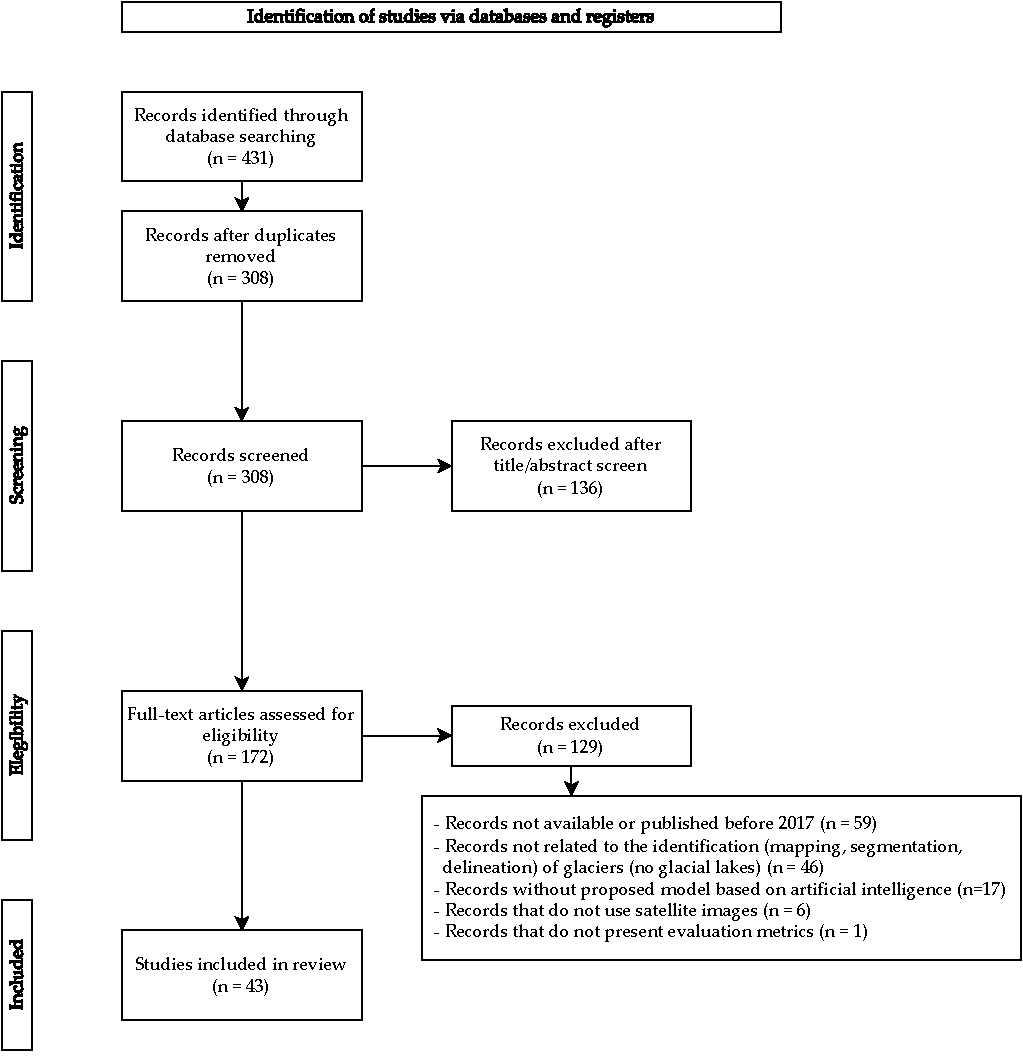
\includegraphics[width=1\textwidth]{images/prisma.pdf}
    \label{fig:prisma}
    \caption{Proceso de búsqueda y selección}
\end{figure}

% =========================================================================
% RESULTADOS Y ANÁLISIS
% =========================================================================

\section{Resultados y análisis}

\begin{figure}[H]
    \centering
    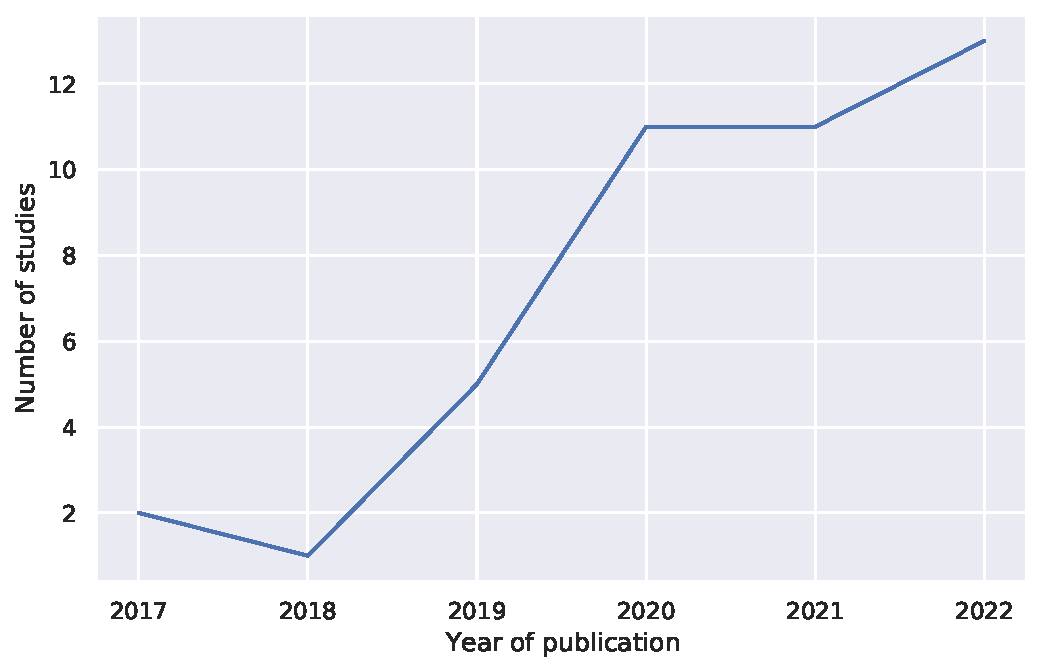
\includegraphics[width=.65\textwidth]{images/fr_years.pdf}
    \label{fig:fr_years}
    \caption{Number of studies by year of publication.}
\end{figure}
En donde se puede identificar un incremento en la publicación de estudios relacionados a la identificación de glaciares en imágenes satelitáles aplicando técncias de inteligencia artificial.



\begin{table}[H]
    \centering
    \caption{Estudios encontrados, duplicados y seleccionados.}
    \hspace{1cm}
    \label{tab:result}
    \begin{tabularx}{\textwidth}{Xccc}
        \hline
        \textbf{Base de datos}  & \textbf{N° encontrados} & \textbf{N° seleccionados} \\ \hline
        {arXiv}                 & 5                       & 1                         \\
        IEEE Xplore             & 15                      & 10                        \\
        MDPI                    & 35                      & 8                         \\
        Nature                  & 27                      & 1                         \\
        Science Direct          & 22                      & 10                        \\
        Scopus                  & 50                      & 5                         \\
        Scopus / Web of Science & 252                     & 3                         \\
        Springer Link           & 16                      & 4                         \\
        Taylor \& Francis       & 9                       & 1                         \\ \hline
        \textbf{TOTAL}          & \textbf{431}            & 43                        \\ \hline
    \end{tabularx}
\end{table}

\begin{figure}[H]
    \centering
    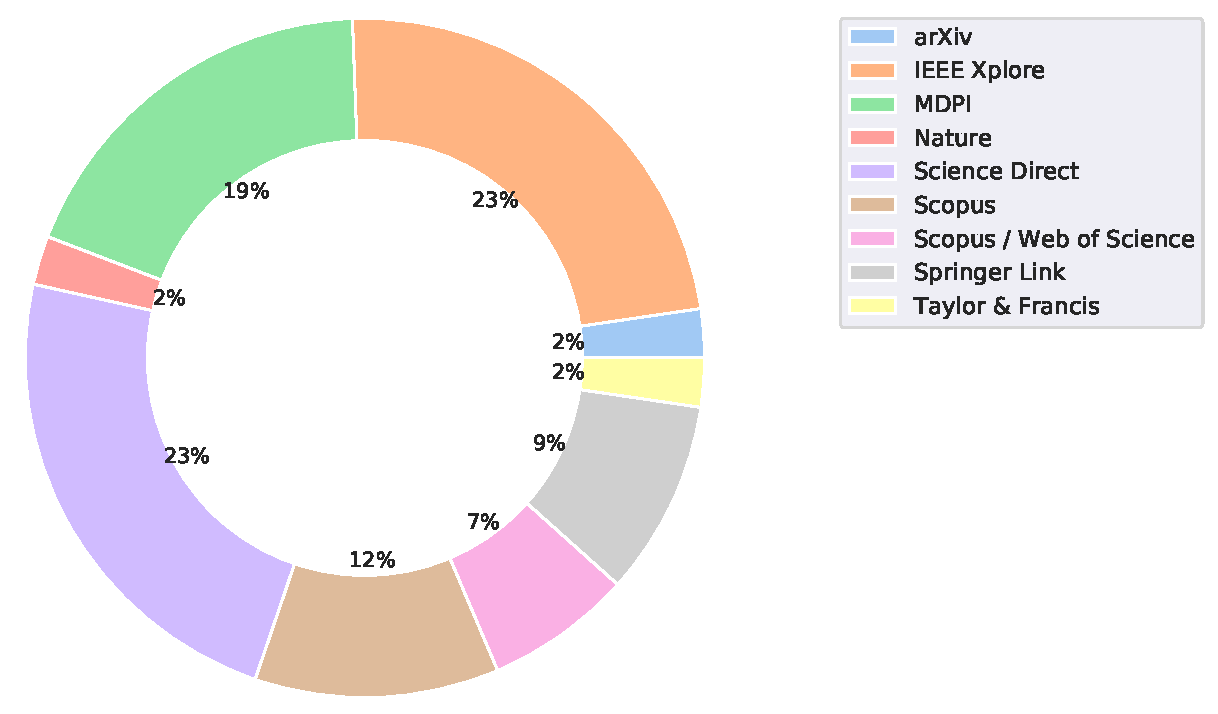
\includegraphics[width=.65\textwidth]{images/fr_publisher.pdf}
    \label{fig:fr_publiser}
    \caption{.}
\end{figure}

\begin{table}[H]
    \centering
    \caption{Estudios encontrados, duplicados y seleccionados.}
    \hspace{1cm}
    \label{tab:result}
    \begin{tabularx}{\textwidth}{Xc}
        \hline
        \textbf{Country} & \textbf{N°} \\ \hline
        China            & 14          \\
        United States    & 9           \\
        Germany          & 8           \\
        India            & 4           \\
        Pakistan         & 2           \\
        Italy            & 1           \\
        Japan            & 1           \\
        Norway           & 1           \\
        Peru             & 1           \\
        Saudi Arabia     & 1           \\
        United Kingdom   & 1           \\  \hline
    \end{tabularx}
\end{table}

\begin{figure}[H]
    \centering
    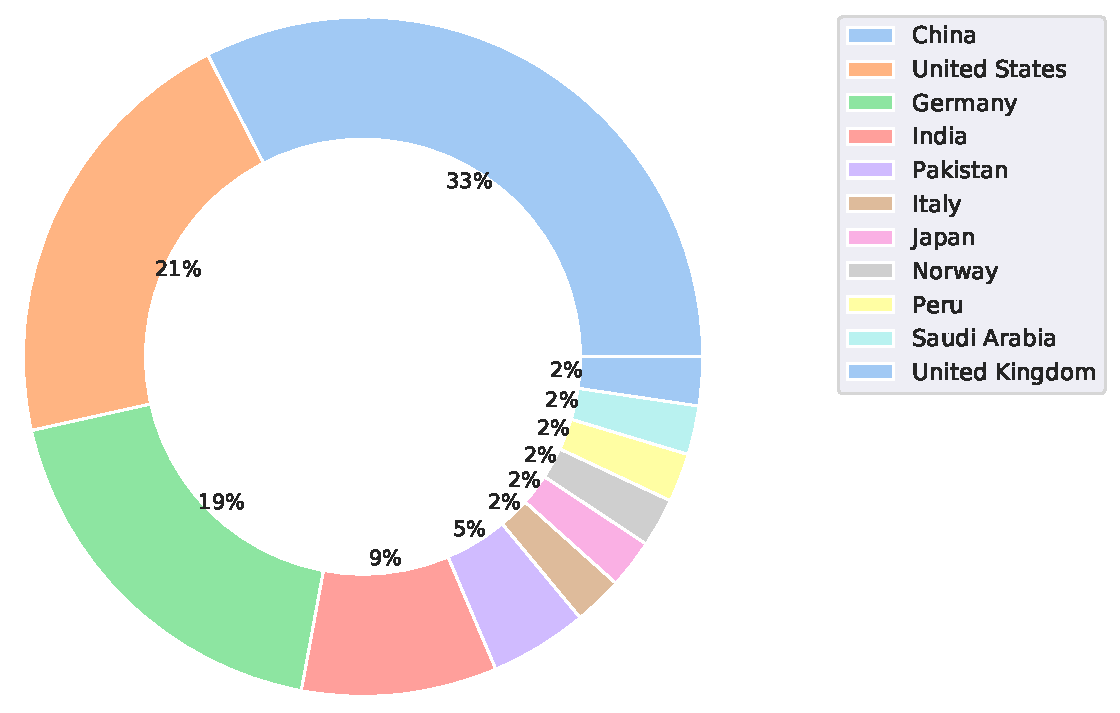
\includegraphics[width=.65\textwidth]{images/fr_country.pdf}
    \label{fig:frog}
    \caption{.}
\end{figure}

\begin{table}[H]
    \centering
    \caption{Estudios encontrados, duplicados y seleccionados.}
    \hspace{1cm}
    \label{tab:result}
    \begin{tabularx}{\textwidth}{Xc}
        \hline
        \textbf{Document type} & \textbf{N°} \\ \hline
        Article                & 34          \\
        Conference Paper       & 9           \\  \hline
    \end{tabularx}
\end{table}

\begin{figure}[H]
    \centering
    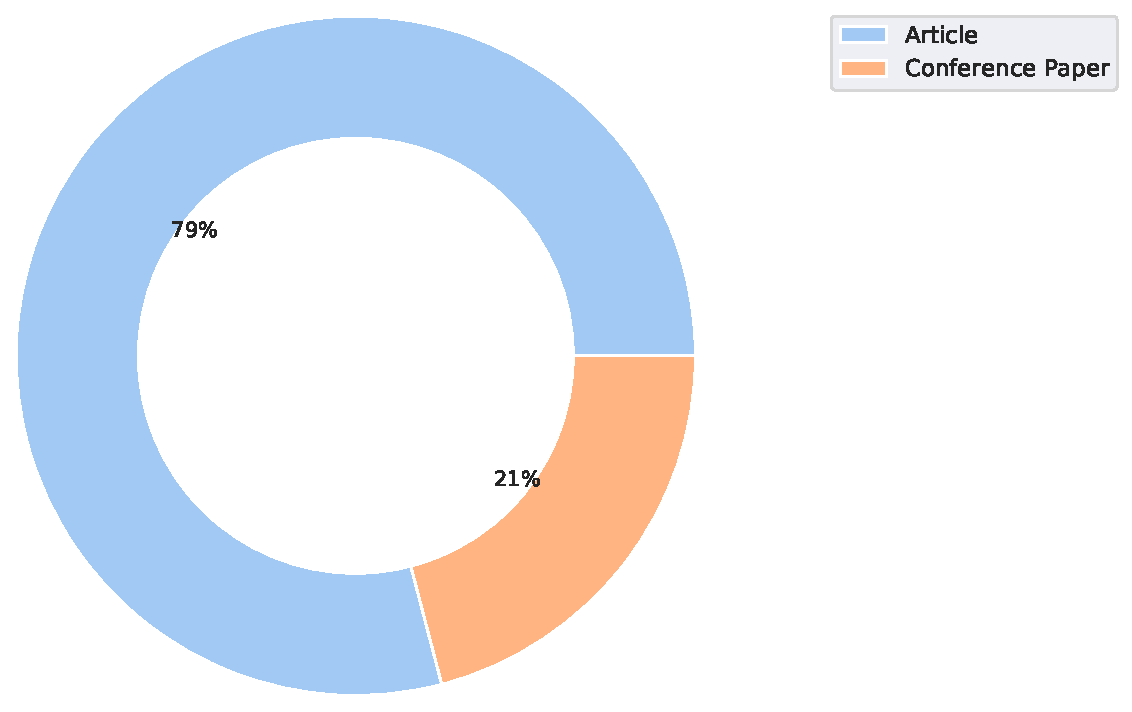
\includegraphics[width=.65\textwidth]{images/fr_document_type.pdf}
    \label{fig:frog}
    \caption{.}
\end{figure}

Asimismo, se hizo una evaluación de los Journal donde fueron publicados los estudios seleccionados, siendo “Remote Sensing” el Journal con más estudios seleccionados (7). En la Tabla 1 se muestra la lista completa de Journals con el respectivo número de estudios.

\begin{table}[H]
    \centering
    \caption{Journals identified as relevant, and number of relevant papers.}
    \hspace{1cm}
    \label{tab:databases}
    \begin{tabularx}{\textwidth}{Xc}
        \hline
        \textbf{Name of journal}                                                           &   \\ \hline
        Remote Sensing                                                                     & 7 \\
        IEEE Access                                                                        & 3 \\
        IEEE Journal of Selected Topics in Applied Earth Observations and Remote Sensing   & 3 \\
        ISPRS, Remote Sensing and Spatial Information Sciences                             & 3 \\
        International Geoscience and Remote Sensing Symposium (IGARSS)                     & 2 \\
        Advances in Space Research                                                         & 2 \\
        International Journal of Applied Earth Observation and Geoinformation              & 2 \\
        Remote Sensing of Environment                                                      & 2 \\
        The Cryosphere                                                                     & 2 \\
        Journal of the Indian Society of Remote Sensing                                    & 2 \\
        NeurIPS 2020 Workshop Tackling Climate Change with Machine Learning                & 1 \\
        Water                                                                              & 1 \\
        IEEE Transactions on Geoscience and Remote Sensing                                 & 1 \\
        Workshop on Hyperspectral Image and Signal Processing, Evolution in Remote Sensing & 1 \\
        Scientific Reports                                                                 & 1 \\
        Ain Shams Engineering Journal                                                      & 1 \\
        Applied Computing and Geosciences                                                  & 1 \\
        Geomorphology                                                                      & 1 \\
        Remote Sensing Applications: Society and Environment                               & 1 \\
        ACM International Conference Proceeding Series                                     & 1 \\
        Cehui Xuebao/Acta Geodaetica et Cartographica Sinica                               & 1 \\
        Frontiers in Earth Science                                                         & 1 \\
        Arabian Journal of Geosciences                                                     & 1 \\
        International Conference on Computer Engineering and Networks                      & 1 \\
        International Journal of Digital Earth                                             & 1 \\ \hline
    \end{tabularx}
\end{table}

\begin{figure}[H]
    \centering
    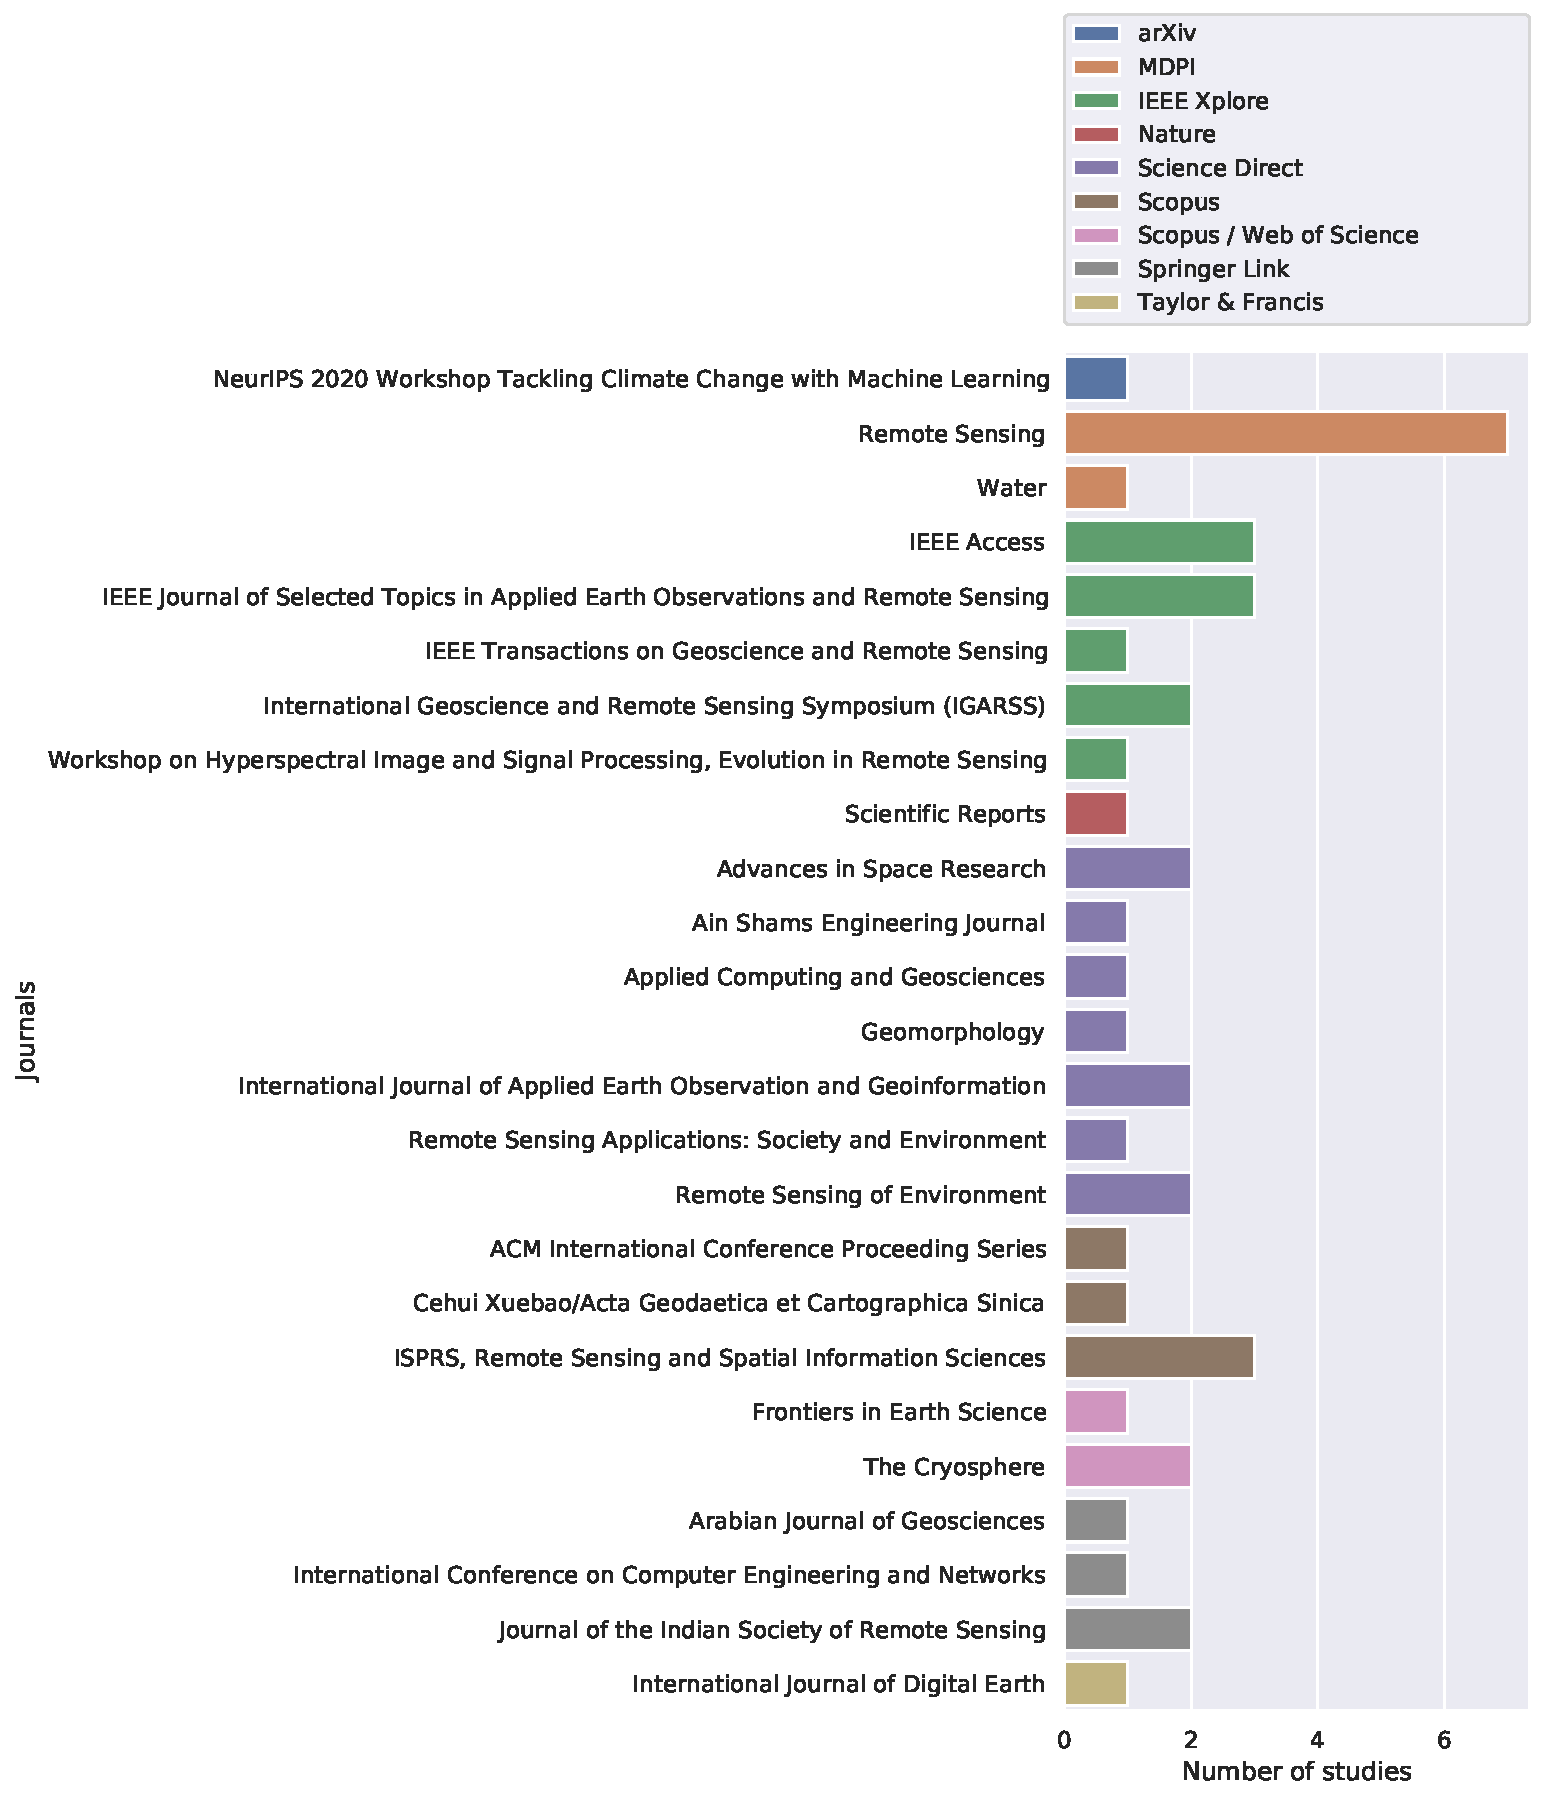
\includegraphics[width=1\textwidth]{images/fr_publisher_journal.pdf}
    \label{fig:frog}
    \caption{.}
\end{figure}



\subsection{RQ1: ¿Qué imágenes satelitales conformaron el conjunto de datos?}

En la teledetección es común emplear datos obtenidos a traves

\cite{zhang2021automated}
\cite{Nijhawan2018}

\subsection{RQ2: ¿Cuántas imágenes satelitales/muestras se utilizaron en la construcción del conjunto de datos?}


\subsection{RQ3: ¿Qué tipo de glaciar se buscó identificar en el estudio?}

\begin{figure}[H]
    \centering
    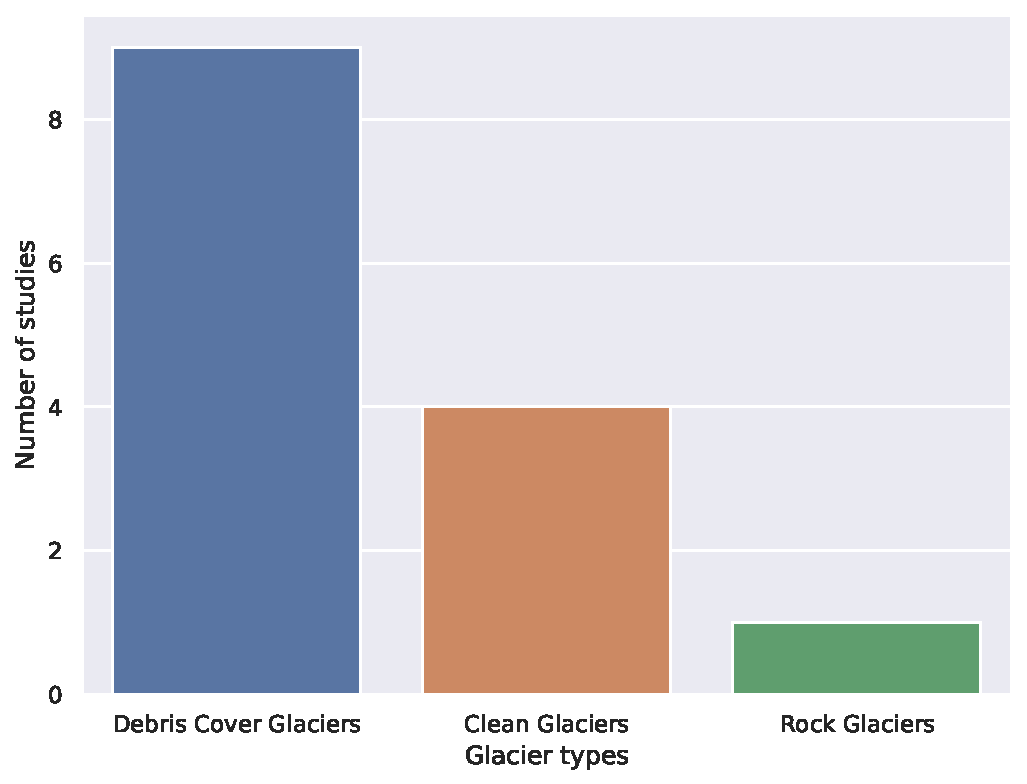
\includegraphics[width=.6\textwidth]{images/fr_glacier_type_1.pdf}
    \label{fig:picoc}
    \caption{Regiones}
\end{figure}

\begin{figure}[H]
    \centering
    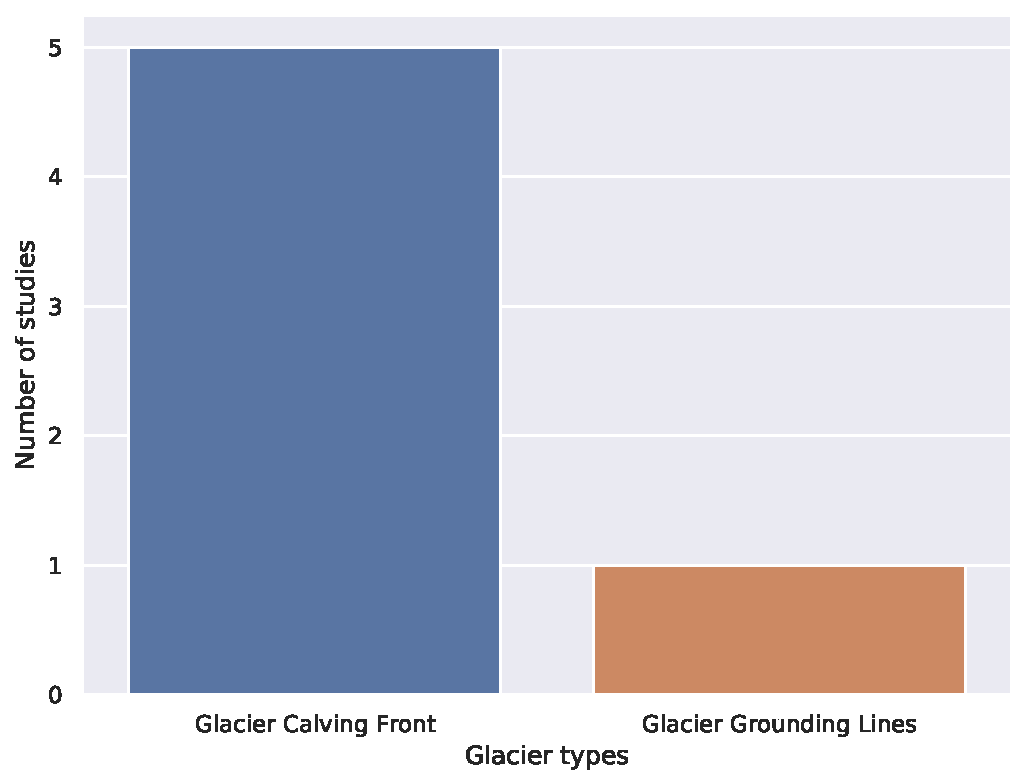
\includegraphics[width=.6\textwidth]{images/fr_glacier_type_2.pdf}
    \label{fig:picoc}
    \caption{Regiones}
\end{figure}

\subsection{RQ4: ¿Cuál es la región geográfica de estudio?}

\begin{figure}[H]
    \centering
    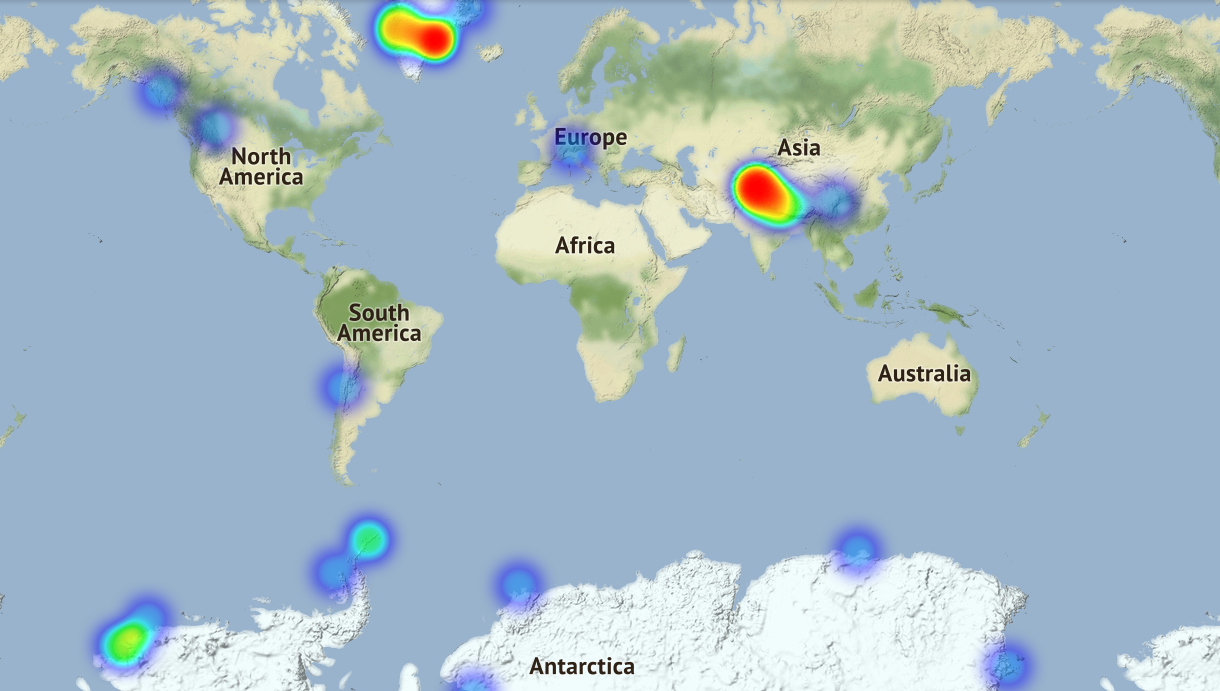
\includegraphics[width=1\textwidth]{images/fr_regions.png}
    \label{fig:picoc}
    \caption{Regiones}
\end{figure}

Las regiones de la Antartida y Groenlandia corresponden a estudios relacionados a la detección de frentes de desprendimiento glaciar en su totalidad.

\subsection{RQ5: ¿Qué algoritmo de inteligencia artificial se empleó como base del modelo propuesto?}


\subsection{RQ6: ¿Cuáles fueron las métricas utilizadas para la evaluación del modelo?}

Las métricas predominantes en

\section{Conclusiones}

\section{Agradecimientos}

\bibliographystyle{IEEEtran}
\bibliography{sample}

\end{document}